\chapter{Introduction}
\label{ch:intro}
%
\section{Motivation}
\label{sec:motivation}
Natural phenomena are a challenging topic in the field of computer graphics.
Actual examples are complex structures which are to be found throughout nature,
such as mountains, trees and water. The latter is especially interesting
because of its highly dynamic form which poses a variety of sophisticated problems.
For computer graphics to reproduce the diverse appearance of ocean surfaces
represents one such problem.
% Scenery with the ocean as its spotlight is wide in range, 
%Figures~\ref{fig:ocean:calm}, \ref{fig:ocean:storm}
%and \ref{fig:ocean:sunset} give examples of the broad visual nature of oceans.
But to cover all the dynamics as well as the lighting of an entire ocean would
exceed the scope of this work.
We may approach a more specific subject, namely the synthesis of animated ocean
surfaces which are both believable and computationally feasible.
Fortunately, the oceanographic research community did already develop models
which satisfy those requirements, as they are essential for oceanographic
simulations. Therefore, we combine consolidated findings from oceanographic
research with computer graphics algorithms to complete the task at hand.
%
% believable ocean surface geometry~\emph{based on} consolidated findings from the
% oceanographic research community.
%
% . We focus our interest on the generation of believable
% ocean surface geometry based on consolidated findings from the oceanographic
% research community.
%
% Based on consolidated findings from the
% oceanographic research community we focus ourselves on the generation of
% believable ocean surface geometry
%
% Hence, our interest focuses on the
% geometry of ocean surfaces using consolidated findings from the oceanographic
% research community.
% 
% In the context of this work we focus our interest on the ocean surfaces.
% 
% In the context of this work we focus our interest on the ever-changing shape of
% ocean surfaces.
% 
% Our interest focuses on the geometry of ocean surfaces using
% consolidated findings from the oceanographic research community.
%
%
%
%\begin{figure}
 %\centering
 %\subtop
 %{
  %\includegraphics[scale=2]{figures/calm300.png}
  %\label{fig:ocean:calm}
 %}
%%\caption{Calm sea under a clear sky. Source:~\cite{misc:noaa:calm}}
 %\subtop
 %{
  %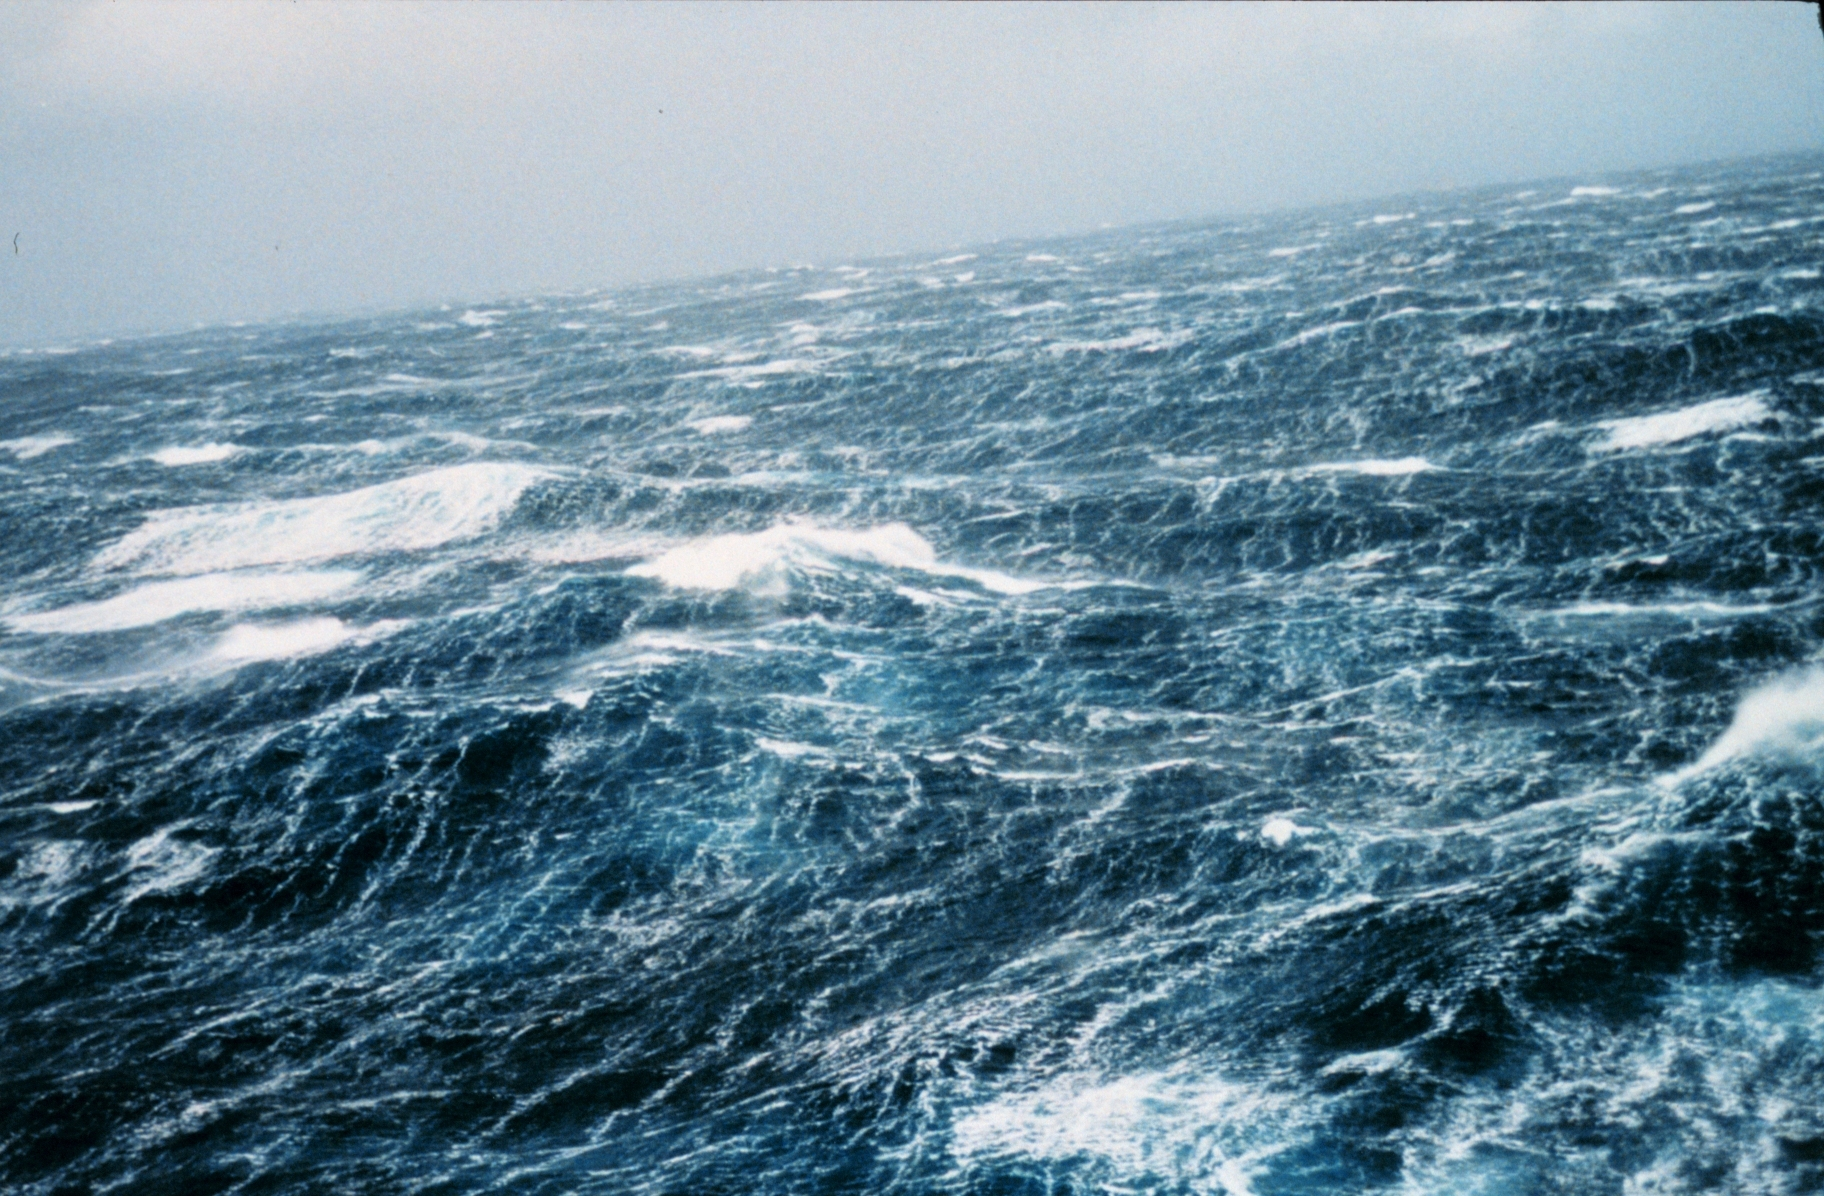
\includegraphics[scale=2]{figures/storm300.png}
%%\caption{Storm waves in the North Pacific. Source:~\cite{misc:noaa:storm}}
  %\label{fig:ocean:storm}
	%}
%\end{figure}
%%
\section{Problem Statement}
\label{sec:problem_statement}
%
Rendering an ocean is a demanding task for several reasons. First, consider the
sheer size of a water body as large as an ocean, which in numerous viewing
situations will be visible all the way to the horizon. Second, the ocean surface
is dynamic, therefore it needs to be constantly updated with the passage of time
even though the wave interactions that define its shape are huge in terms of complexity.
% thus we employ approximative models. %published by the oceanographic research community.
Third, the optics of water are intricate. Incoming light may be reflected at the
surface or may be refracted into the water body, where the ratio between both is
dependent on the angle of incidence between the incoming light and the surface
normal at the point of incidence. Some of the refracted light may find its way
back to the ocean's surface, either by scattering inside the water body or by
reflection at the sea bottom, or possibly by a combination of both. Moreover,
waves on the ocean surface may break and cause surf and foam,
both of which strongly deviate in appearance from the surrounding water surface.
%both of which interact with light drastically different than the surrounding water surface.
%
%  adding another
% layer of detail to the visual appearance of the ocean surface.
%
% The visual appearance of an ocean
% surface is highly dependent on its surroundings, because it reflects light from various
% sources e.g the sun, the skydome, clouds, as well as objects close to the
% water surface, such as boats and ships. Water does not only reflect light, it
% also refracts light, where the amount of refracted light to find its way back
% to the water surface is highly dependent on the depth of the water body.
% Moreover, the particulets contained inside the water body interact with the
% refracted light and therefore may cause a tint of the ocean surface.
% In addition, waves may break and cause surf and foam. Both interact with light
% drastically different than the surrounding water surface, adding another layer
% of detail.
%
%
%  (reflections), the depth of the underlying
% water body (refractions), as well as on the particulets contained in the water
% body itself (scattering).
% 
% The generation and animation of a water surface as large as an ocean is a demanding
% task. In most situations will often span all the way to the horizon, 
% 
% Some light is reflected, some is
% refracted, where the latter may or may not find its way back to the water
% surface.
%
\begin{figure}[p]
\centering
\includegraphics[width=0.75\textwidth]{figures/p1020149.jpg}
\caption{
	Karre, Julie (Photographer).
	(2013, August 7).
	One of the last sunsets for the first leg of the Oregon II [digital image].
	Retrieved from~\cite{misc:noaa:sunset}.
	}
\label{fig:ocean:sunset}
\end{figure}
\begin{figure}[p]
\centering
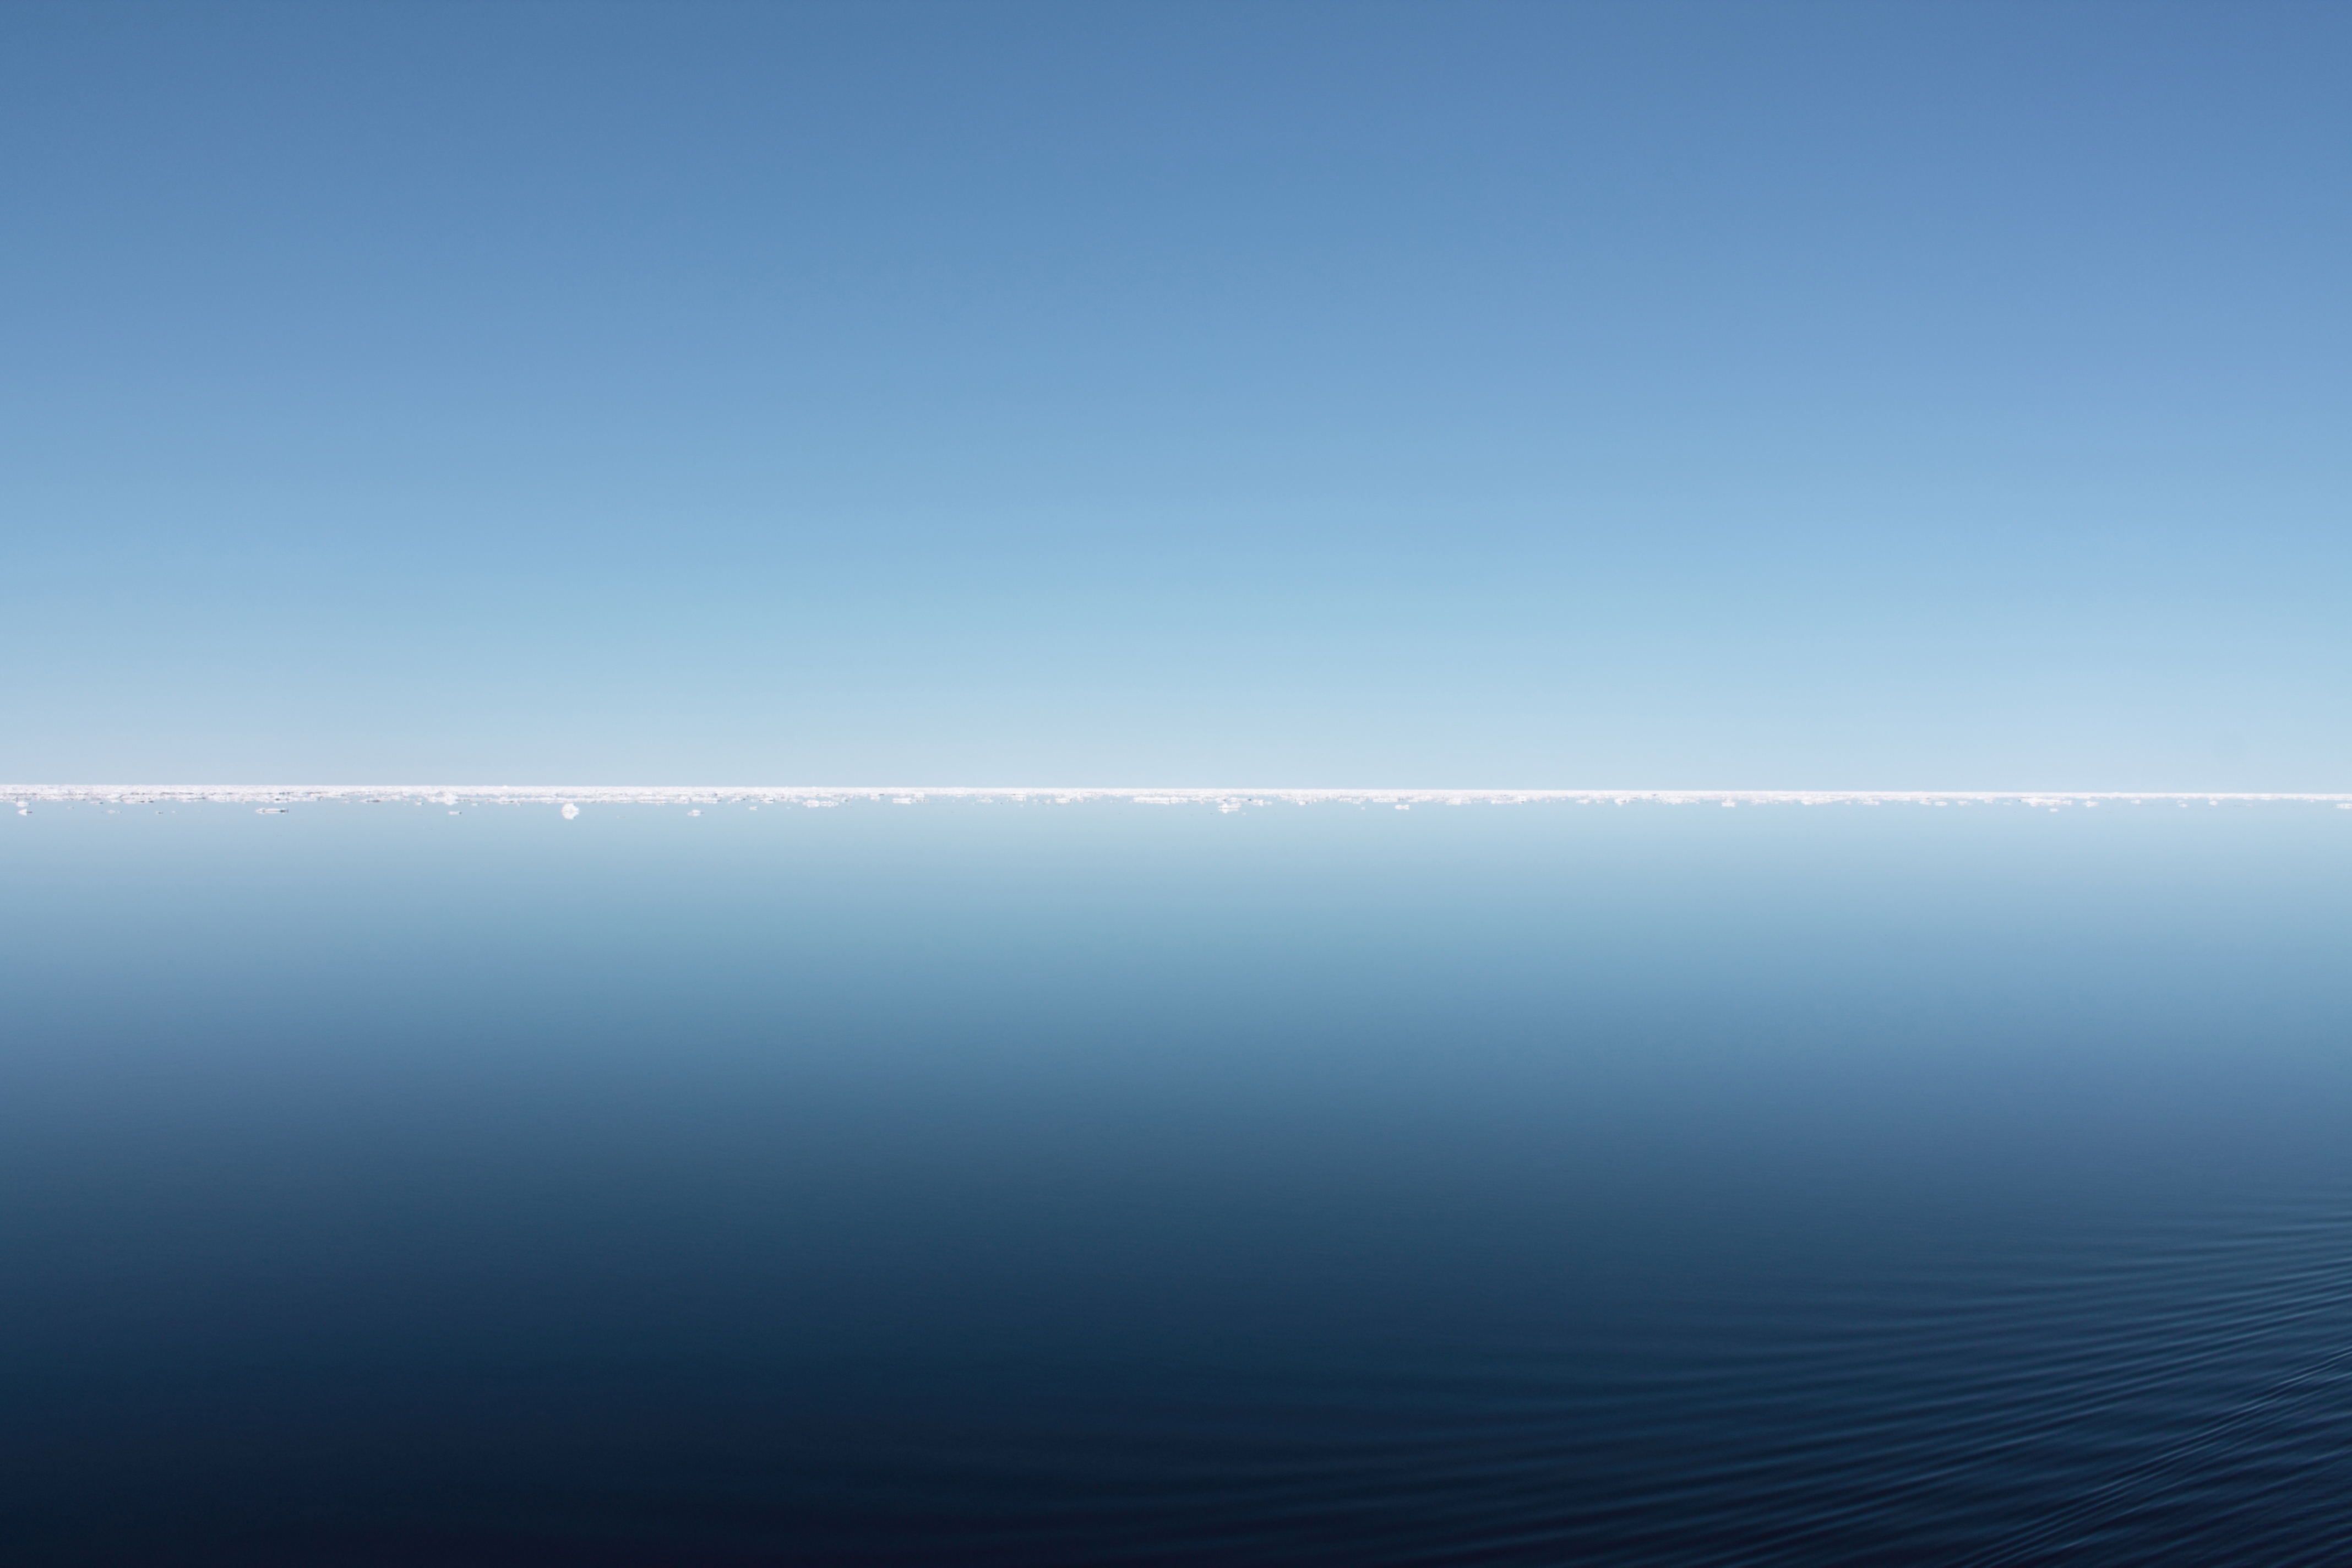
\includegraphics[width=0.75\textwidth]{figures/helen-smith-arcticsea.jpg}
\caption{
	Smith, Helen (Photographer).
	(2013, June 4).
	A stunningly blue and calm Arctic reflection of sea and sky divided by distant
	bright white ice and interrupted by ripples created by the ship. 15th June
	2012 on the RRS James Clark Ross in the Arctic sea ice between Svalbard and
	Greenland [digital image].
	Retrieved from~\cite{misc:noaa:arctic}.
	}
\end{figure}
\begin{figure}
\centering
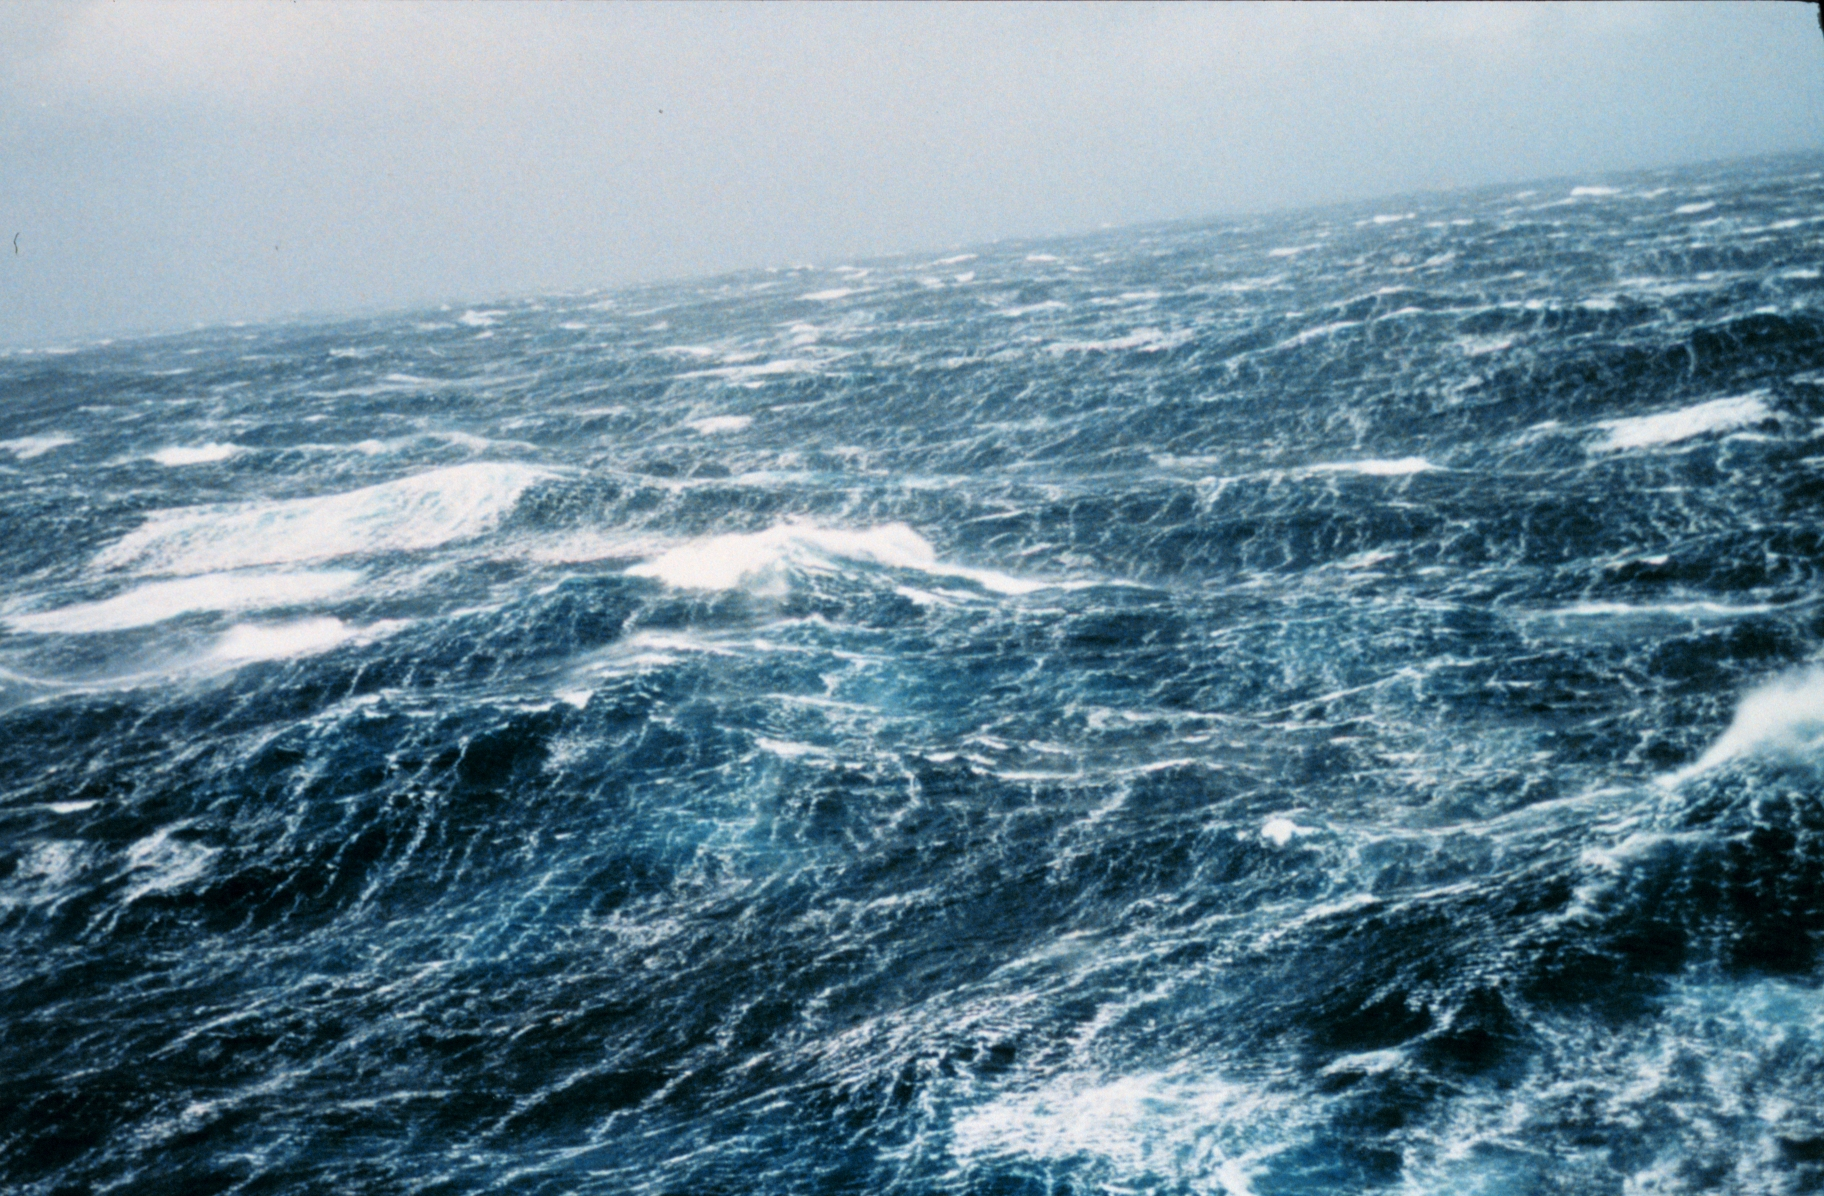
\includegraphics[width=0.75\textwidth]{figures/wea00816.jpg}
\caption{
	National Oceanic and Atmospheric Administration (Photographer).
	(1989, Winter).
	North Pacific storm waves as seen from the M/V NOBLE STAR [digital image].
	Retrieved from~\cite{misc:noaa:storm}.
	}
\end{figure}
%
%
\section{Scope and Focus of the Work}
\label{sec:scope_and_focus}
The scope of this thesis includes the generation, animation and rendering of the
surface of an open ocean in real-time. We focus our interest on the synthesis of
animated ocean surface geometry, for which we will adopt a set of mathematical
models from oceanographic research. Specific properties of said models allow for
easy addition and reduction of detail, as well as for a range of algorithmic
optimisations. The former combined with the latter gives us the opportunity to
strike a well-adjusted balance between model detail and computational workload,
and thereby to improve upon the status quo of current implementations.
%
% Note: The oceanographic models discussed in this work are not based on fluid
% dynamics, hence, convincing interaction between the ocean surface and other
% objects is beyond the scope of this thesis.
%
\section{Structure of the Work}
\label{sec:structure}
The remainder of this work is organized as follows: Chapter
\ref{ch:state_of_the_art} gives a survey of existing ocean simulation and
rendering methods. Chapter~\ref{ch:background} elaborates on the theoretical
background the oceanographic models are based on, as well as on the models
themselves. Chapter~\ref{ch:implementation} describes in detail the
synthesis of all data related to the ocean surface, including both the algorithmic
optimisations and the level of detail mechanism. Furthermore, we give an overview
of the rendering algorithms adopted for our implementation. In Chapter
\ref{ch:summary} we summarize our work and discuss the improvements we were able
to achieve in comparison to the state of the art. Moreover, we will suggest
future work based on open issues of our implementation.
